%!TeX root=main.tex
\begin{section}{Observations}
	We created 11 sample test cases of small graphs of around 2-10 nodes ranging from a weighted $C_5$ to a $P_4$.  We individually verified each case and concluded that they were correct. \\
	
	\begin{subsection}{PACE Dataset Observations}
	We then ran our program on the testcases in the PACE dataset. We were able to run 14 tests successfully within the time limit of 30 minutes. \\
	
	We were only able to run tests with $k \leq 6$. All other testcases had a higher treewidth. This is because the bag size becomes $8$, and the join node takes up a lot of computation time because we go through all $B(k)$ partitions pairwise to compute their acyclic merges. When the bag size is 9, $B(k) = 21147$, where $\binom{B(9)}{2}$ is huge to store in memory (takes around 700MB). Hence, reading and writing from this pre computed structure takes a lot of time on our PCs. \\
	
		We believe with a dedicated engine (like an online judge), our performance would be better. \\
	
		It's worth noting that the participants in the actual PACE 2018 Challenge, either implemented the $O(2^k)$ algorithm or implemented the current algorithm, but switched to a more efficient one when the treewidth crossed a certain threshold. \\
	
	\begin{figure}
		\centering
		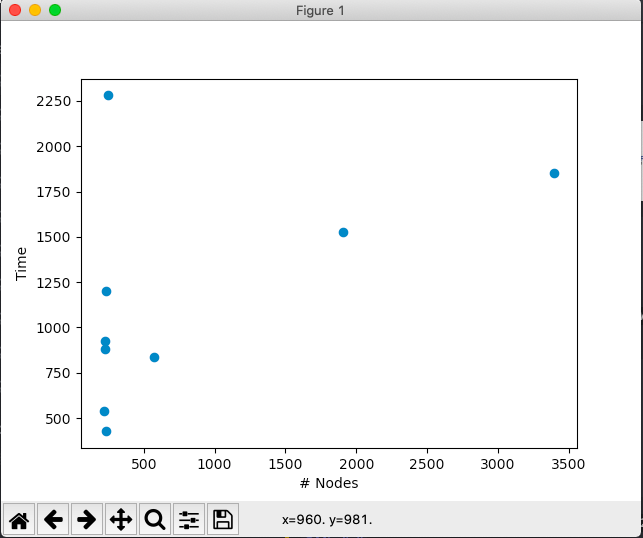
\includegraphics[scale=0.5]{NodeGraph.png}
		\caption{Plot of $|V(G)|$ vs time}
		\label{fig:nodegraph}
	\end{figure}

	While analysing the amount of time each testcase (instances 6 - 14 from PACE 2018 dataset), we realised that while the time taken to compute the optimal weight increased as the graph size increased, there was no direct relation showing so. As it can be seen in Fig. \ref{fig:nodegraph}, there are small graphs which have similar sizes (around 250 vertices) but tend to take different times. \\
	
	Since this was unusual, we ended up plotting different graphs for edges vs time and vertices * edges vs time to see if there was any difference and there wasn't. These plots looked like Fig. \ref{fig:nodegraph}. \\
	
	Our next hypothesis was that since Join Nodes tend to take more time to compute, there might be more join nodes in the graphs which take more time. This is because the treewidth is the same amongst the test cases we are considering. However, even this plot looked exactly like Fig. \ref{fig:nodegraph}. \\
	
	The reason was that while the treewidth is the same for all graphs, the join nodes in some graphs could have a smaller bag size than some other graphs. Hence, graphs with more join nodes with bigger bag sizes (but limited by treewidth) should take more time. To compute this, we summed up $|B|^|B|$ over all bags $B$ of the Join Nodes in the nice tree decomposition. We got the graph in Fig. \ref{fig:joingraph}. As we can see, there is a clear increase in time as this weighted sum increases. This also shows that the running time is asymptotically $O(k^O(k))$.  \\
	
	\begin{figure}
		\centering
		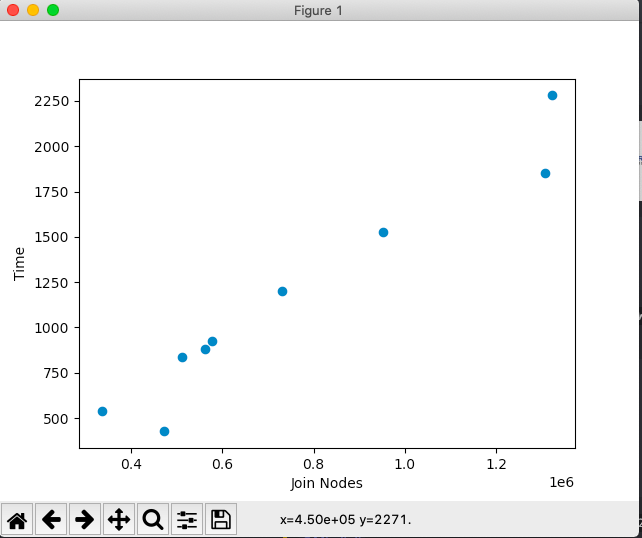
\includegraphics[scale=0.5]{JoinGraph}
		\caption{Weighted sum of Join Nodes vs time}
		\label{fig:joingraph}
	\end{figure}
	

	\end{subsection}

	This algorithm could not be tested on the track A dataset since the tree decompositions weren't given. 
	
\end{section}